\chapter{Interfaz de usuario}
\label{ch:diseño_interfaz_usuario}

\section{Guía de estilo}

A la hora de llevar a cabo el diseño de las interfaces de usuario se realizó una definición del estilo gráfico que tendría la aplicación y que se debería seguir para conseguir consistencia entre todas las pantallas de la misma. La base de la guía de estilo son \textbf{las directrices de Material Design} (véase \fref{ssec:guia_material_design}). Sobre esas bases se decidieron también los siguientes puntos:

\begin{itemize}
    \item El color principal de la aplicación será el \emph{dodger blue} (\code{\#29b6f6}).
    \item El color secundario de la aplicación será su complementario, el \emph{selective yellow} (\code{\#ffb300}).
    \item La aplicación ofrecerá temas claro y oscuro. Por defecto se mostrará acorde al tema del sistema operativo del usuario.
    \item Se utilizarán tarjetas para mostrar la información personal de los usuarios. 
    \begin{itemize}
        \item El nombre del usuario es la información mínima a mostrar inicialmente en la tarjeta.
        \item La información adicional de contacto estará en el anverso de la tarjeta o en una extensión desplegable, se usará la alternativa que más convenga a cada situación.
        \item Las dos alternativas se usarán con botones situados en el lado derecho de la tarjeta.
    \end{itemize}
    \item Todos los botones de navegación ofrecerán un icono y un texto indicando el destino.
    \item Los elementos de la interfaz como los botones o tarjetas tendrán bordes redondeados.
    \item Los errores se comunicarán por medio de \emph{toasts} al usuario.
    \item Todos los elementos utilizarán colores definidos en el tema de la aplicación.
\end{itemize}

\subsection{Tema de color}

El tema de color fue generado con la herramienta de que Material ofrece para tal empresa, \textbf{\nameref{ssec:color_tool}} (\fref{ssec:color_tool}), a partir de los dos colores que fueron seleccionados como colores base de la aplicación. La paleta de colores resultante fue la siguiente:

\begin{table}[H]
    \centering
    \begin{tabular}{|l|c|}  \hline
        \textbf{Color}         & \textbf{RGB} \\ \hline
        Primario         & \code{\#29b6f6} \\
        Primario claro         & \code{\#73e8ff} \\
        Primario oscuro        & \code{\#0086c3} \\ 
        Secundario         & \code{\#ffb300} \\ 
        Secundario claro         & \code{\#ffe54c} \\ 
        Secundario oscuro         & \code{\#c68400} \\ 
        Texto primario         & \code{\#000000} \\ 
        Texto secundario         & \code{\#212121} \\ 
        Superficie         & \code{\#eaf4f6} \\ \hline
    \end{tabular}
    \caption{Paleta de colores de la aplicación}
    \label{tab:paleta_colores}
\end{table}

\subsection{Icono de la aplicación}

El icono de la aplicación (\fref{fig:app_icon}) está basado en el lema principal y nombre de la aplicación, el \emph{"Todos para uno y uno para todos"},  que ya se comentó en el \fref{sec:justification}, y en el concepto de vínculos entre pacientes y cuidadores. 

El icono está compuesto por otros dos iconos que representan a su vez a los dos tipos de usuarios de la aplicación: los \textbf{Pacientes} (\fref{fig:patient_icon}) y los \textbf{Cuidadores} (\fref{fig:keeper_icon}). Los primeros son el punto central alrededor del que gira este sistema y su icono representa esto, un entidad central que recibe la ayuda exterior de sus cuidadores. Los Cuidadores por otro lado se representan como esas entidades exteriores que orbitan alrededor del Cuidador y que al hacerlo establecen vínculos entre sí, pues la base de esta aplicación radica también la cooperación entre Cuidadores. Los dos iconos superpuestos representan el entramado que se teje en \emph{All For One}, una cadena de socorro mutuo entre Pacientes y Cuidadores.

\vspace{30pt}
\begin{figure}[H]
    \centering
    \begin{minipage}{0.25\textwidth}
        \centering
        
\includegraphics[width=0.5\textwidth]{Diseño/patient-icon.png}
        \caption{Icono de Paciente}
        \label{fig:patient_icon}
    \end{minipage}\hfill
    \begin{minipage}{0.25\textwidth}
        \centering
        
\includegraphics[width=0.5\textwidth]{Diseño/keeper-icon.png}
        \caption{Icono de Cuidador}
        \label{fig:keeper_icon}
    \end{minipage}\hfill
    \begin{minipage}{0.25\textwidth}
        \centering
        
\includegraphics[width=0.5\textwidth]{Diseño/4l1-icon.png}
        \caption{Icono de AllForOne}
        \label{fig:app_icon}
    \end{minipage}
\end{figure}

\section{Logo de la aplicación}

Además del icono también se creó un logo que permita identificar la aplicación de una forma más descriptiva y representativa, pues estará compuesto del nombre de la aplicación. La base de su diseño es el propio nombre de la aplicación y, por tanto, el lema de la misma. El logo (\fref{fig:app_logo}) es un \textbf{All} escrito con los colores del tema, los cuales distinguen también un \textbf{4} sobre la letra \emph{A} y un \textbf{1} bajo la letra \emph{L} del final. Esto nos deja: \textbf{ALL-4-1}, lo cuál leído en inglés tiene una lectura similar al nombre de la aplicación: \textbf{All For One.}

\begin{figure}[H]
    \centering
    
\includegraphics[width=0.5\textwidth]{images/Diseño/4l1-logo.png}
    \caption{Logo de la aplicación}
    \label{fig:app_logo}
\end{figure}

\section{Launch}

\begin{figure}[H]
    \centering
    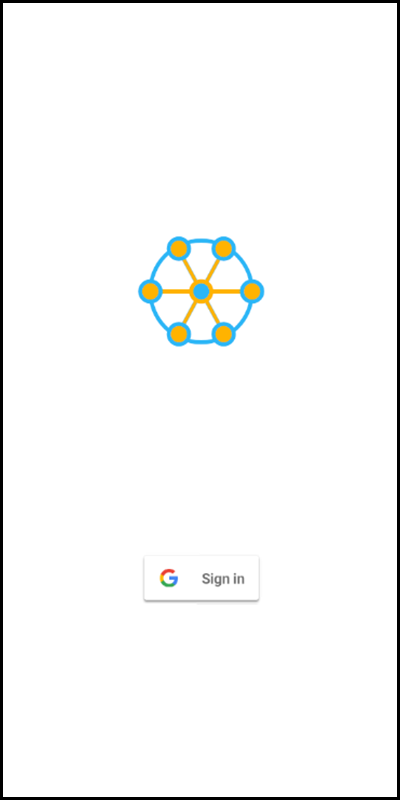
\includegraphics[width=0.25\textwidth]{Diseño/CapturaLaunch.png}
    \caption{Diseño de la pantalla de lanzamiento}
    \label{scr:launch}
\end{figure}

La pantalla de lanzamiento (\fref{scr:launch}) ofrece una única funcionalidad, \textbf{el inicio de sesión} con la cuenta de Google del usuario., por ello la pantalla contará únicamente con un botón para llevar a cabo esa acción. El botón en cuestión debe ser el servido por la propia biblioteca de autenticación de Google para ofrecer familiaridad al usuario y transmitir rápidamente que el inicio de sesión usa ese servicio. Aparte de dicho botón se dispondrá el icono de la aplicación para que el usuario sepa qué aplicación está empleando por si se inicia o accede a ella de forma indirecta. Hay margen para otros posibles añadidos como podrían ser la marca de registro o la versión de la aplicación.

\section{Set Up}

\begin{figure}[H]
    \centering
    \begin{minipage}{0.20\textwidth}
        \centering
        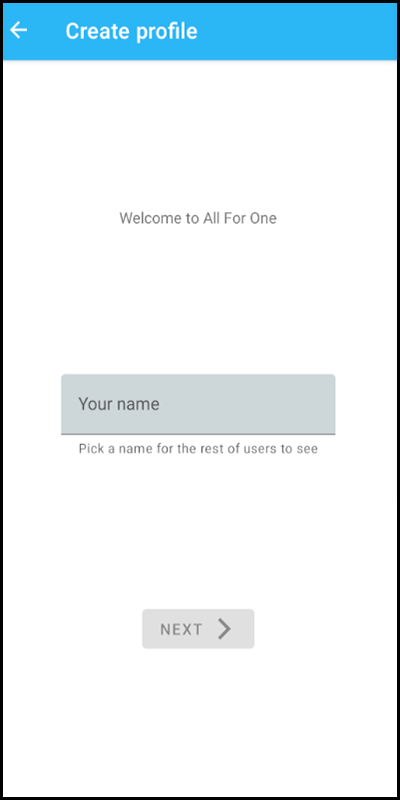
\includegraphics[width=1\textwidth]{Diseño/CapturaSetUpA.png}
        \caption{Diseño de la pantalla de configuración de nombre}
        \label{scr:setup_name}
    \end{minipage}\hfill
    \begin{minipage}{0.20\textwidth}
        \vspace{-18pt}
        \centering
        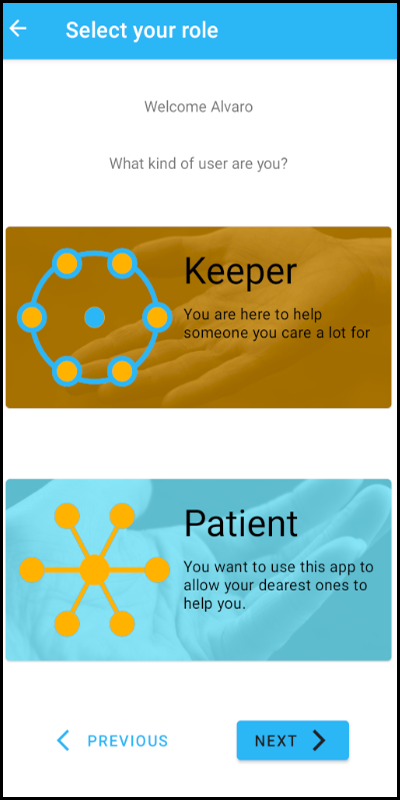
\includegraphics[width=1\textwidth]{Diseño/CapturaSetUpB.png}
        \caption{Diseño de la pantalla de elección de rol}
        \label{scr:setup_role}
    \end{minipage}\hfill
    \begin{minipage}{0.20\textwidth}
        \centering
        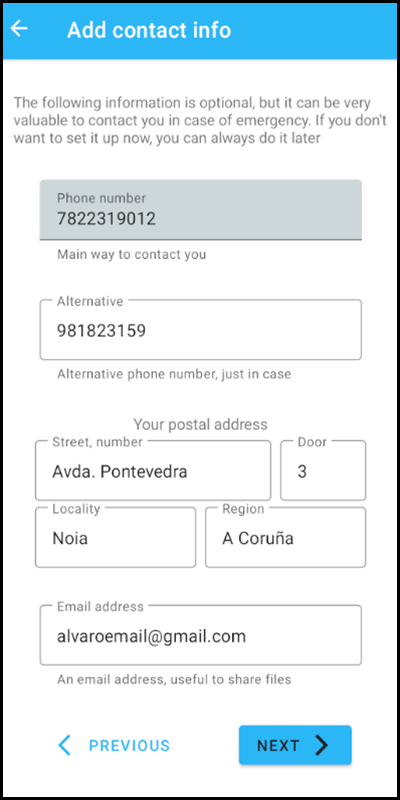
\includegraphics[width=1\textwidth]{Diseño/CapturaSetUpC.png}
        \caption{Diseño de la pantalla de introducción de datos}
        \label{scr:setup_contact}
    \end{minipage}\hfill
    \begin{minipage}{0.20\textwidth}
        \centering
        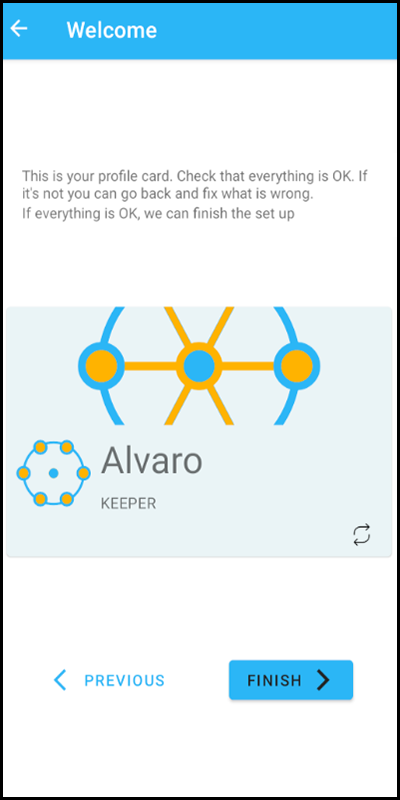
\includegraphics[width=1\textwidth]{Diseño/CapturaSetUpD.png}
        \caption{Diseño de la pantalla de confirmación del perfil}
        \label{scr:setup_confirmation}
    \end{minipage}\hfill
\end{figure}

La pantalla de configuración del perfil será la pantalla a la que accedan los nuevos usuarios que intenten iniciar sesión por primera vez. Esta pantalla estará compuesta por cuatro distintas, una para cada etapa del proceso con tendrán botones para avanzar o retroceder entre ellas. 

La primera de estas pantallas es la de \textbf{configuración del nombre} (\fref{scr:setup_name}), donde habrá un campo de texto en el que el usuario podrá introducir el nombre que lo represente. A esta pantalla le sigue la de \textbf{selección del rol} ( \fref{scr:setup_role}), que ofrecerá dos tarjetas representando las opciones.

Una vez seleccionado el rol, el usuario progresará a otra pantalla (\fref{scr:setup_contact}) donde podrá rellenar sus \textbf{datos de contacto} en los distintos campos de texto que se le dispondrán para tal acción. Tras completar todos estos pasos la única pantalla restante será la de \textbf{confirmación del perfil} (\fref{scr:setup_confirmation}). En esta última pantalla se mostrará la tarjeta de perfil del usuario con los datos que ha introducido de forma que pueda ver todo de nuevo de forma sencilla antes de terminar el registro.

\section{Main}

\begin{figure}[H]
    \centering
    \begin{minipage}{0.5\textwidth}
        \centering
        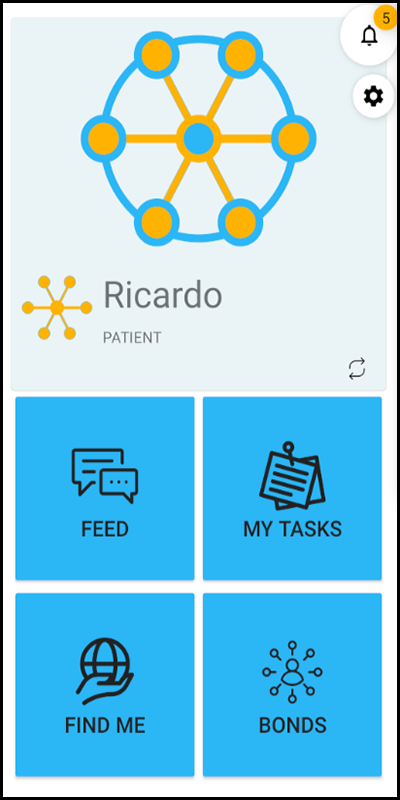
\includegraphics[width=0.5\textwidth]{Diseño/CapturaMainA.png}
        \label{scr:main}
    \end{minipage}\hfill
    \begin{minipage}{0.5\textwidth}
        \centering
        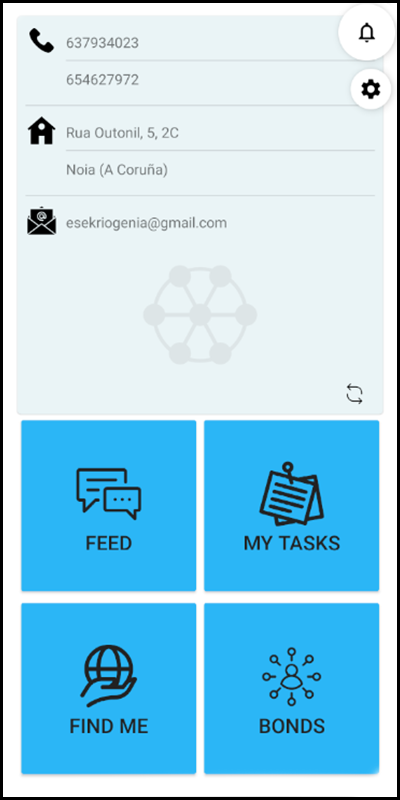
\includegraphics[width=0.5\textwidth]{Diseño/CapturaMainB.png}
        \label{scr:main_b}
    \end{minipage}\hfill
    \caption{Diseño de la pantalla principal}
\end{figure}

La pantalla principal es el punto de navegación principal de la aplicación y da acceso al resto de funciones de la aplicación. Al ser el también el punto de entrada tras el inicio de sesión es un lugar idóneo para situar \textbf{los datos del Paciente}, de forma que el acceso a los mismos requiera el menor esfuerzo posible de memoria, facilitando el acceso a ellos a los usuarios con los síntomas de la enfermedad. La tarjeta es voltaeable por medio del botón situado en su esquina inferior derecha.

Las cuatro grandes funciones principales de la aplicación (el feed de comunicación, la gestión de tareas, la geolocalización y la consulta de vínculos) serán accesibles a través de los \textbf{cuatros grandes botones} situados bajo la tarjeta del Paciente. Al ser las funciones principales cuenta con un acceso más resaltable que los demás puntos de navegación de la pantalla.

Esos otros dos puntos de navegación son el acceso a las notificaciones y a los ajustes. Los botones a los mismos no cuentan con el relleno del color principal y están situados en la esquina superior derecha, lugar habitual de localización para estas funciones. El acceso a las notificaciones contará además con una chapa indicando \textbf{el número de notificaciones} no leídas que tiene el usuario, indicando así si es necesario desplegar dicha pantalla.

\section{Feed}

\begin{figure}[H]
    \centering
    \begin{minipage}{0.5\textwidth}
        \centering
        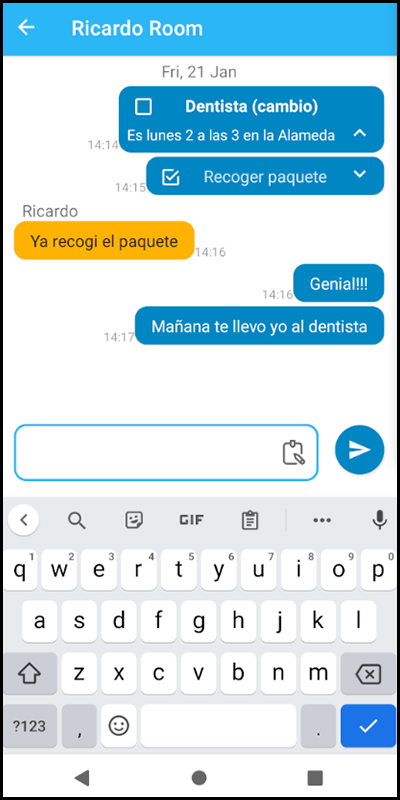
\includegraphics[width=0.5\textwidth]{Diseño/CapturaFeed.png}
        \label{scr:feed}
    \end{minipage}\hfill
    \begin{minipage}{0.5\textwidth}
        \centering
        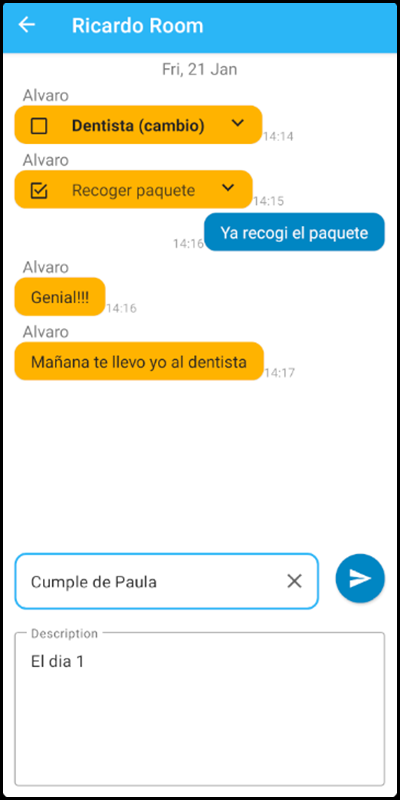
\includegraphics[width=0.5\textwidth]{Diseño/CapturaFeedTarea.png}
        \label{scr:feed_task_mode}
    \end{minipage}\hfill
    \caption{Diseño de la pantalla de feed}
\end{figure}

El diseño de la pantalla del feed (\fref{scr:feed}) es similar a los diseños habituales de \textbf{pantallas de chat}. En el lado derecho y en azul se mostrarán los mensajes usados por el propio usuario y a la izquierda se listarán los mensajes enviados por los usuarios asociados con el nombre del usuario que lo envió. Como en los diseños habituales, en la parte inferior se ofrecerá un campo de texto para escribir y enviar el mensaje con el botón de su derecha.

Todos los mensajes mostrarán la hora de envío de los mismos y se agruparán por fecha de envío. Las tareas se mostrarán como mensajes de texto pero incluyendo además una casilla representando su estado y una flecha que permita desplegar la descripción de la tarea. Las tareas ya completas se verán con un color de texto más apagado para que sean fácilmente distinguibles a primera vista.

Una diferencia que tendrá esta pantalla de feed respecto a otros chats será el \textbf{modo crear tarea}. Este se mostrará usando el botón con forma de portafolios del interior del campo de texto. Al usarlo el icono cambiará a una X que sirva para cerrarlo y una campo de texto mayor se abrirá en la parte inferior de la pantalla para poder introducir la descripción. El envío de estas será con el mismo botón que los mensajes de texto.

\section{Tasks}

\begin{figure}[H]
    \centering
    \begin{minipage}{0.45\textwidth}
        \centering
        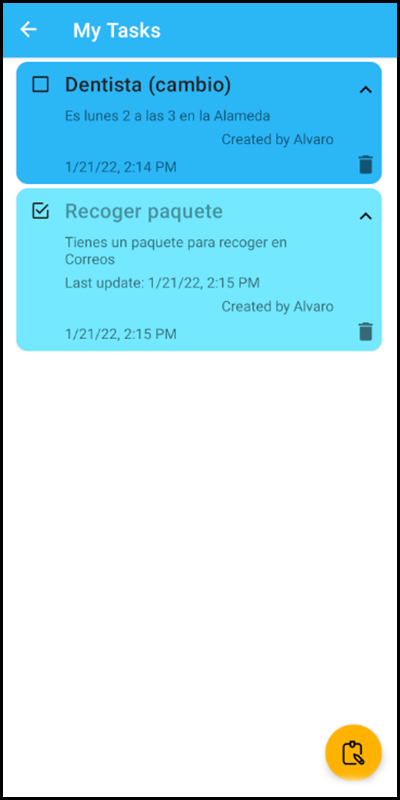
\includegraphics[width=0.5\textwidth]{Diseño/CapturaTareas.png}
        \caption{Diseño de la pantalla de tareas}
        \label{scr:task}
    \end{minipage}\hfill
    \begin{minipage}{0.45\textwidth}
        \centering
        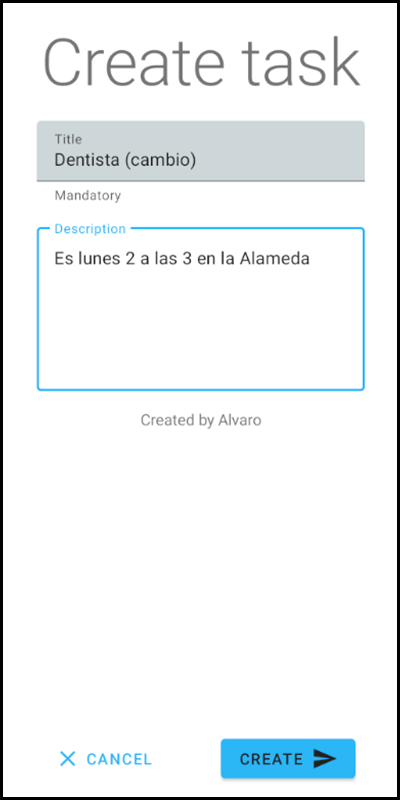
\includegraphics[width=0.5\textwidth]{Diseño/CapturaTareasCrear.png}
        \caption{Diseño de la pantalla de crear tarea}
        \label{scr:task_crear}
    \end{minipage}\hfill
\end{figure}

La pantalla de tareas (\fref{scr:task}) lista las tareas en tarjetas con el título, una casilla con el estado de la tarea, el autor de la misma y la fecha de creación de la tarea. Más información como la descripción o el último momento de actualización se mostrarán al desplegar los datos de la tarea con la flecha de la tarjeta para tal uso. Las tareas ya completas tendrán color y texto más claro, por lo que a simple vista \textbf{podrán diferenciarse los dos tipos de tarea}. La casilla del estado será también un botón que se pueda usar para cambiar el estado de la tarea, además de este botón habrá otro para eliminarlas. 

Finalmente, la pantalla también tendrá un botón para desplegar la pantalla de \textbf{creación de tareas} (\fref{scr:task_crear}). En dicho diálogo habrá un campo de texto para introducir el título y otro para rellenar la descripción. La creación de la tarea se podrá confirmar o cancelar con los botones que este diálogo tendrá en la parte inferior.

\section{Location}

\begin{figure}[H]
    \centering
    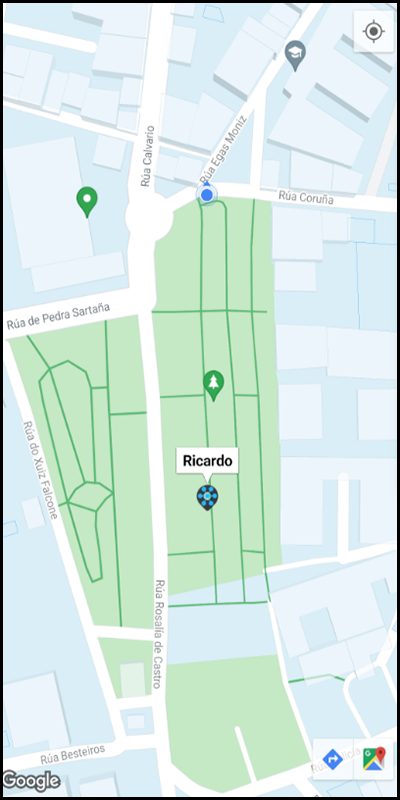
\includegraphics[width=0.2\textwidth]{Diseño/CapturaLocalización.png}
    \caption{Diseño de la pantalla de geolocalización}
    \label{scr:location}
\end{figure}

La pantalla de geolocalización (\fref{scr:location}) es una \textbf{actividad con un mapa} que ocupa toda la actividad similar a muchos otros servicios. Los colores del mapa de Google Maps se ofrecerán modificados para que vayan más acordes a los colores de la aplicación. En esa pantalla se mostrará la posición del usuario con un círculo azul con un cono visión. Marcadores de distintos colores representarán las posiciones del resto de usuarios asociados conectados. Pulsar en esos marcadores mostrará el nombre del usuario al que pertenece.

\section{Bonds}

\begin{figure}[H]
    \centering
    \begin{minipage}{0.5\textwidth}
        \centering
        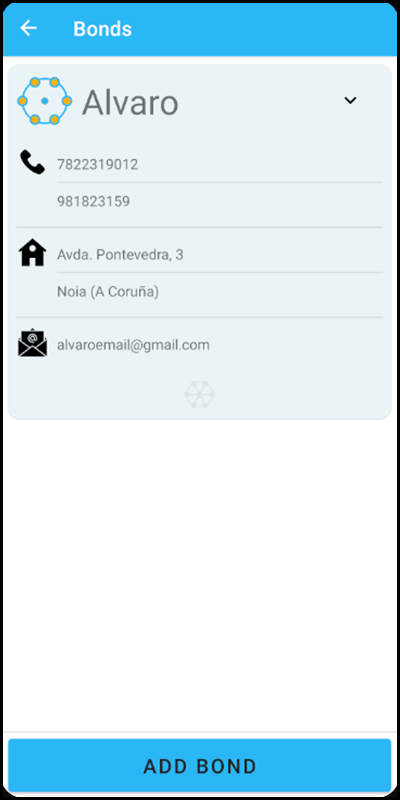
\includegraphics[width=0.45\textwidth]{Diseño/CapturaBondList.png}
        \label{scr:bonds}
    \end{minipage}\hfill
    \begin{minipage}{0.5\textwidth}
        \centering
        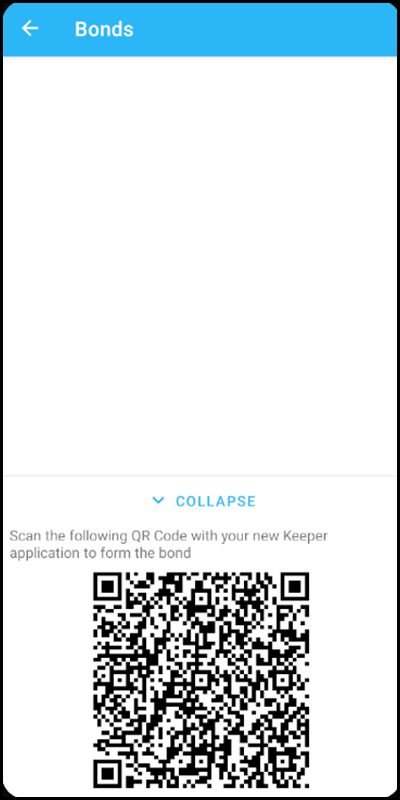
\includegraphics[width=0.45\textwidth]{Diseño/CapturaBoundB.png}
        \label{scr:bonds_qr}
    \end{minipage}\hfill
    \caption{Diseño de la pantalla de vínculos}
\end{figure}

La función de acceso a los vínculos se servirá en una pantalla (\fref{scr:bonds}) que listará los vínculos. Cada uno de estos vínculos \textbf{será una tarjeta} con el nombre del usuario que podrá ser desplegada para mostrar los datos de contacto. Los pacientes, además, tendrán un botón en la parte inferior que les permitirá desplegar un nuevo código QR con un \gls{token} de vinculación como se puede ver en \fref{scr:bonds_qr}.

\section{Scanner}

\begin{figure}[H]
    \centering
    \begin{minipage}{0.45\textwidth}
        \centering
        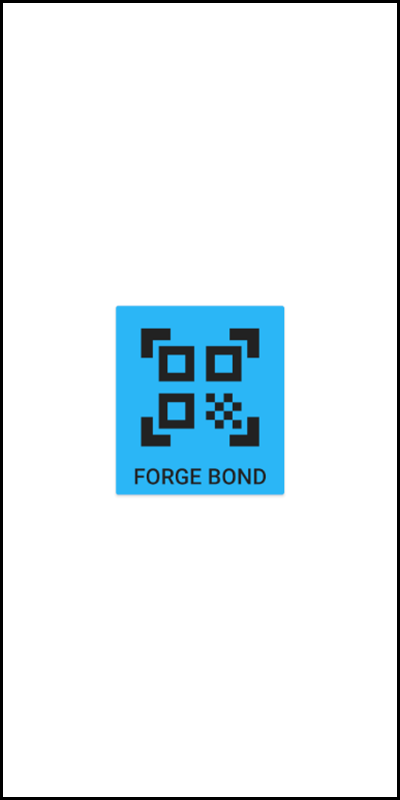
\includegraphics[width=0.5\textwidth]{Diseño/CapturaBoundA.png}
        \caption{Diseño de la pantalla principal sin vínculo}
        \label{scr:unbonded}
    \end{minipage}\hfill
    \begin{minipage}{0.45\textwidth}
        \centering
        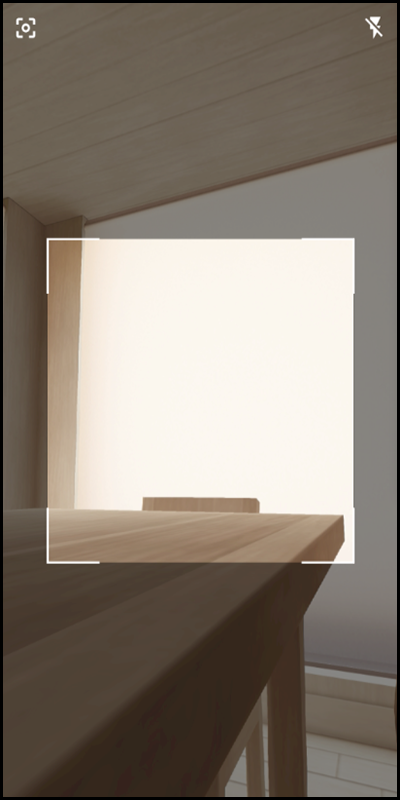
\includegraphics[width=0.5\textwidth]{Diseño/CapturaScanner.png}
        \caption{Diseño de la pantalla de escáner}
        \label{scr:scanner}
    \end{minipage}\hfill
\end{figure}

Para completar los vínculos se debe escanear el código QR, lo que se hace en la pantalla de escáner (\fref{scr:scanner}) a la que se podrán acceder los \textbf{Cuidadores no vinculados} a través de su actividad principal, que se mostrará como se ve en \fref{scr:unbonded}, con únicamente un botón para abrir el escáner. El susodicho escáner será una pantalla ocupada por completo por la cámara en la que estará oscurecida la sección en la que no podrá enfocarse el código.

\section{Notifications}

Las notificaciones se desplegarán y mostrarán en una pantalla como la mostrada en \fref{scr:notifications}. Dicha pantalla listará las acciones a notificar agrupadas según la fecha en la que sucedieron y en un orden de más recientes a más antiguas. Cada notificará contará con un botón con el icono de un ojo para marcar esa notificación como vista. Aparte de ese botón habrá otro en la parte superior para \textbf{marcar todas como vistas}. Por último, las notificaciones relacionadas con alguna pantalla o acceso que se deba visitar contarán con un botón para navegar hasta dicho lugar de la aplicación.



\begin{figure}[H]
    \centering
    \begin{minipage}{0.4\textwidth}
        \centering
        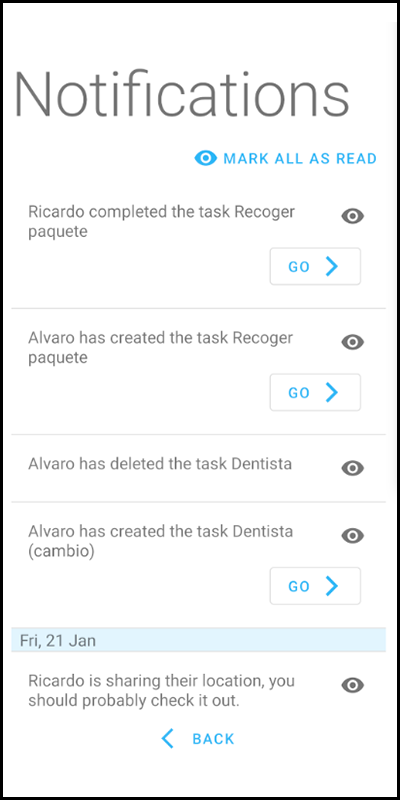
\includegraphics[width=0.5\textwidth]{Diseño/CapturaNotificaciones.png}
        \caption{Diseño de la pantalla de notificaciones}
        \label{scr:notifications}
    \end{minipage}\hfill
    \begin{minipage}{0.4\textwidth}
        \centering
        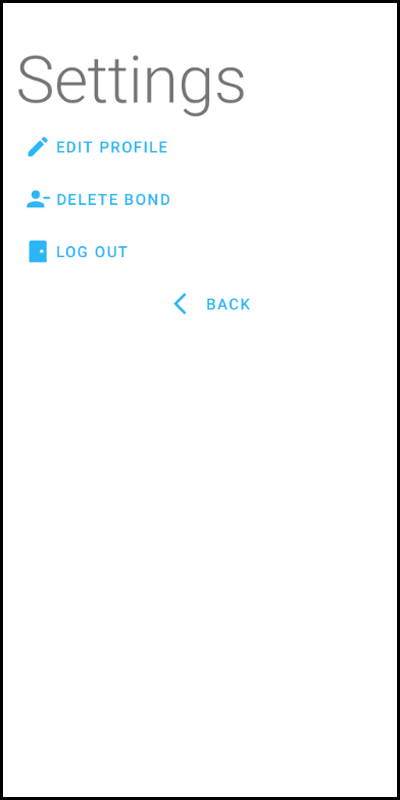
\includegraphics[width=0.5\textwidth]{Diseño/CapturaAjustes.png}
        \caption{Diseño de la pantalla de ajustes}
        \label{scr:settings}
    \end{minipage}\hfill
\end{figure}

\section{Settings}

Las opciones, al igual que las notificaciones, será un diálogo a pantalla completa que se abrirá desde la pantalla principal. Será como la \fref{scr:settings}. En esta pantalla se listarán las posibles opciones del usuario. La opción de \textbf{editar usuario} desplegará campos de texto de las diferentes propiedades del usuario para que este pueda editarlas, lo cuál confirmará con un botón que también se desplegará con la misma opción. El resto de opciones serán también botones, y habrá uno más para cerrar el diálogo y retornar a la pantalla principal.

\section{Mapa de navegación}

El mapa de navegación definitivo con las pantallas recién mostradas es el ilustrado en \fref{scr:navigation}. Las pantallas con fondo azul requieren inicio de sesión y las que tienen fondo verde son exclusivas de los Cuidadores no vinculados.

La navegación comienza siempre en LaunchActivity. Si el usuario no está registrado avanzará a SetUpActivity a través de sus cuatro fragmentos en orden. Si está registrado o si completa el registro a través de SetUpActivity avanzará a MainActivity, desde donde se navegarán al resto de actividades y a los diálogos de notificaciones y ajustes. 

Se ha intentando reducir los pasos de navegación al mínimo y por ello prácticamente todas las funcionalidades son accesibles con una única navegación desde la pantalla principal. A excepción del diálogo de crear tarea, que debe accederse desde TasksActivity.

\begin{figure}[H]
    \centering
    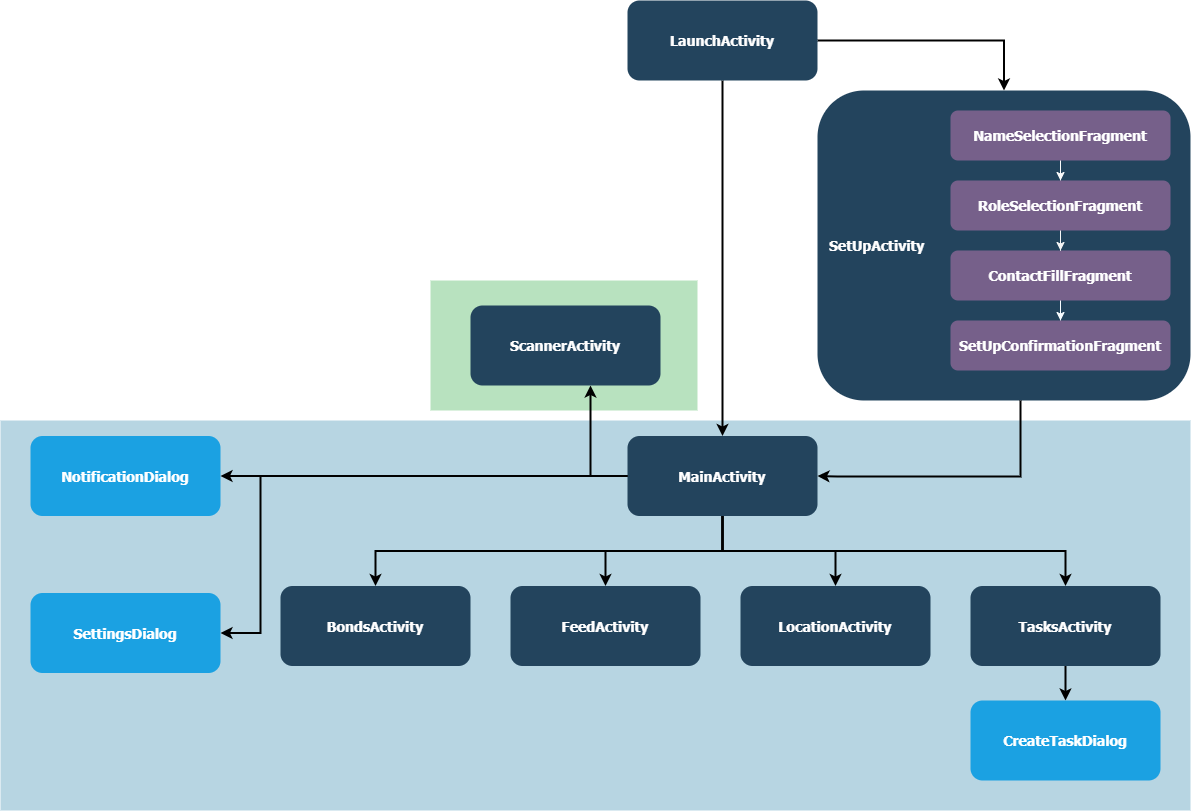
\includegraphics[width=1\textwidth]{Diseño/MapaNavegacionDiseño.drawio.png}
    \caption{Mapa de navegación}
    \label{scr:navigation}
\end{figure}